\subsection{Bảo mật tầng HTTP -- Helmet, CORS, Rate Limit và HTTPS}

Tầng HTTP là điểm tiếp xúc đầu tiên giữa cử tri và hệ thống, do đó các biện pháp phòng thủ tại tầng này được áp dụng đồng thời theo nhiều khía cạnh: \textit{tăng cường bảo mật tiêu đề HTTP} qua Helmet, giới hạn nguồn gốc qua CORS, giới hạn tần suất yêu cầu qua Rate Limiting, ngắt các yêu cầu vượt quá thời gian xử lý qua Timeout, và mã hóa truyền tải qua HTTPS.

\textbf{Helmet:} BFF và Reveal-Vote đều dùng thư viện \pkg{helmet} với cấu hình phân biệt theo môi trường (Hình~\ref{fig:helmet-config}). \textit{Content-Security-Policy} ở chế độ nghiêm ngặt với \pkg{default-src 'none'}, chỉ cho phép \pkg{connect-src 'self'} và buộc nâng cấp HTTP sang HTTPS. Các tiêu đề khác như \pkg{X-Frame-Options}, \pkg{X-Content-Type-Options}, \pkg{Referrer-Policy}, \pkg{Strict-Transport-Security}, \pkg{Cross-Origin-Opener-Policy} đều được bật mặc định.

\begin{figure}[H]
    \centering
    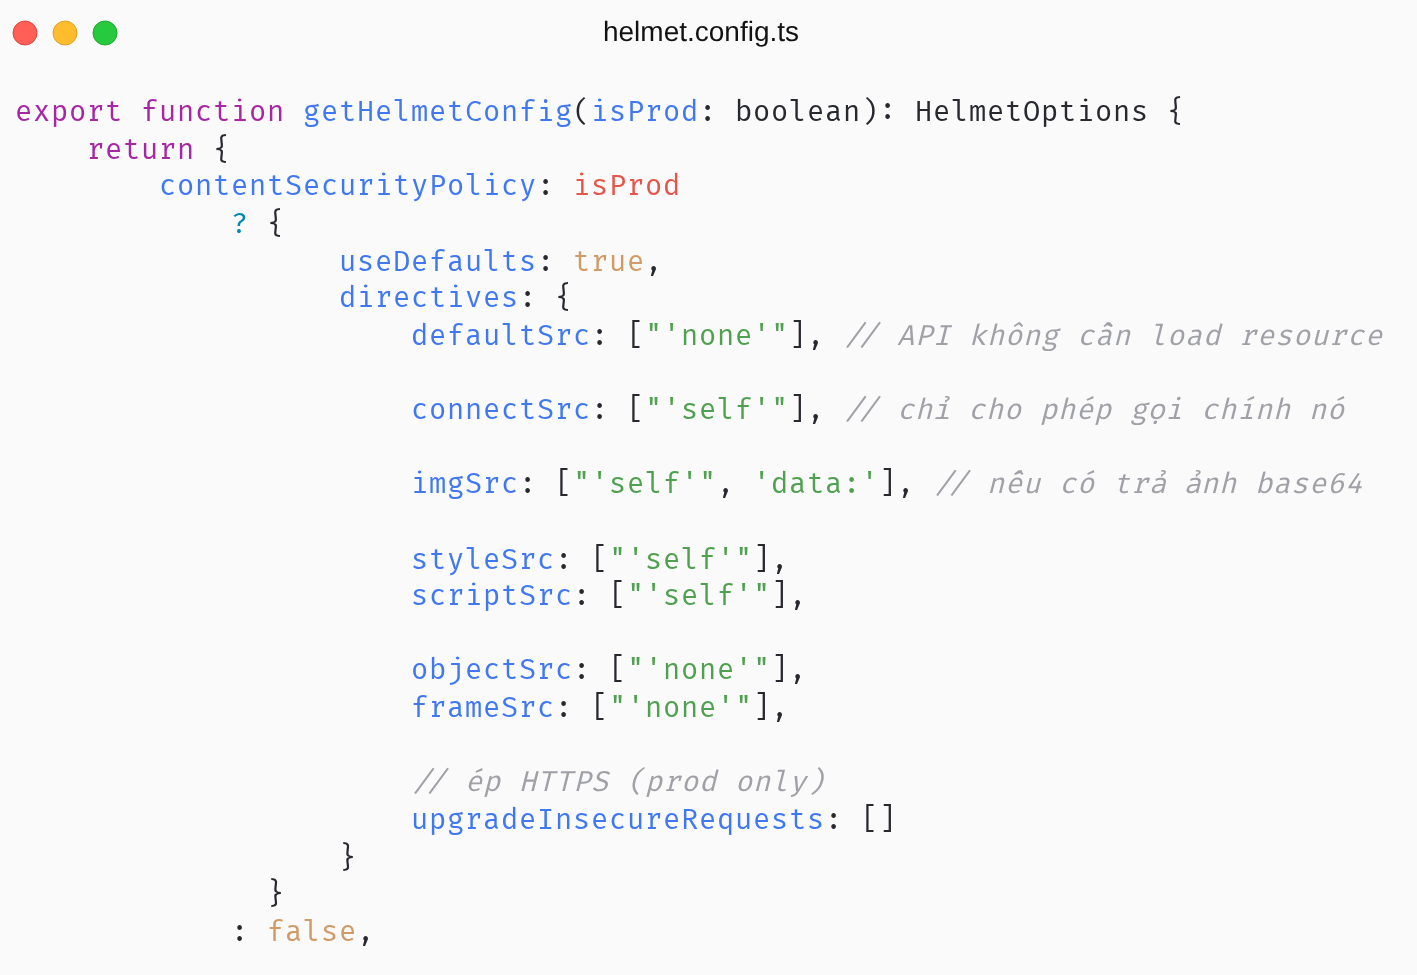
\includegraphics[width=0.85\textwidth, keepaspectratio]{Figures/code/helmet-config.png}
    \caption{Cấu hình Helmet cho môi trường sản xuất}
    \label{fig:helmet-config}
\end{figure}

\textbf{CORS:} Tiêu đề \pkg{Access-Control-Allow-Origin} chỉ chấp nhận các tên miền nằm trong biến môi trường \pkg{CORS\_ORIGINS}. Phương thức được phép giới hạn ở \pkg{GET}, \pkg{POST}, \pkg{PUT}, \pkg{PATCH}, \pkg{DELETE}, \pkg{OPTIONS}, kèm \pkg{credentials} để cookie phiên hợp lệ cho các tên miền tin cậy. Cấu hình này ngăn các trang web bên ngoài gọi API qua \pkg{XMLHttpRequest} hay \pkg{fetch} và đảm nhận một phần vai trò chống CSRF.

\textbf{Rate Limiting:} \pkg{HttpThrottlerGuard} giới hạn 100 yêu cầu mỗi IP trong mỗi 60 giây.

\textbf{Request Timeout:} \pkg{TimeoutInterceptor} áp dụng toán tử \pkg{timeout(5000)} của RxJS cho mọi yêu cầu -- sau 5 giây hệ thống trả về \pkg{408 Request Timeout} thay vì giữ kết nối vô thời hạn. Cơ chế này quan trọng khi peer Fabric phản hồi chậm: yêu cầu của cử tri không bị treo, cho phép họ thử lại thay vì chờ đợi không xác định.

\textbf{HTTPS cho BFF và Reveal-Vote:} Hai dịch vụ đều được phục vụ qua HTTPS. Hệ thống áp dụng mô hình \textit{TLS termination at edge}: một reverse proxy Cloudflare đứng trước, đảm nhận giải mã TLS rồi chuyển tiếp yêu cầu HTTP đến backend trong mạng nội bộ tin cậy. Cách triển khai này tận dụng phần cứng tăng tốc TLS của reverse proxy và giúp việc luân chuyển chứng chỉ trở nên đơn giản -- chỉ phải cập nhật tại một điểm. Trường hợp triển khai trên một máy chủ duy nhất, NestJS hỗ trợ bật HTTPS trực tiếp như sau:

\begin{figure}[H]
    \centering
    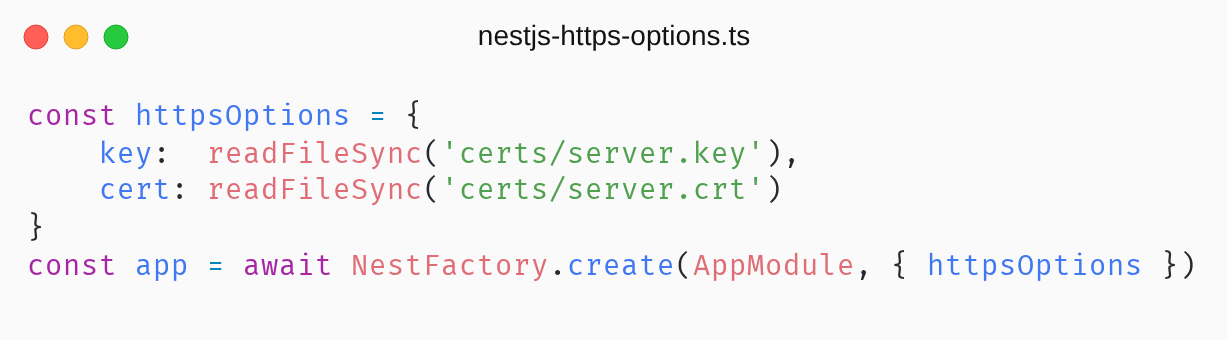
\includegraphics[width=0.70\textwidth, keepaspectratio]{Figures/code/nestjs-https-options.png}
    \caption{Khởi tạo NestJS với httpsOptions để bật HTTPS trực tiếp}
    \label{fig:nestjs-https-options}
\end{figure}
